% !TEX TS-program = lualatex

% Основано на презентации Анны Игоревны Васениной и Владимира Александровича Кутуева
\documentclass[aspectratio=169]{beamer}

%%% Setup fonts.
\usepackage{fontspec}
%% Fancy fonts
\setmainfont{Iosevka Etoile}
\setsansfont{Iosevka Aile}
\setmonofont{Iosevka}

%% Default fonts
% \setmainfont{CMU Serif}
% \setsansfont{CMU Sans Serif}
% \setmonofont{CMU Typewriter Text}

%% Math
\usepackage{amsmath, amsfonts, amsthm, mathtools} % Advanced math tools.
\usepackage{amssymb}

\usepackage{unicode-math} % Allow TTF and OTF fonts in math and allow direct typing unicode math characters.
\unimathsetup{
    warnings-off={
            mathtools-colon,
            mathtools-overbracket
        }
}
% \setmathfont{Lete Sans Math}[CharacterVariant={3,6},StylisticSet={4}]
\setmathfont{Latin Modern Math}

%%% Language settings.
\usepackage{polyglossia}
\setdefaultlanguage{russian}
\setotherlanguage{english}

%%% Beamer settings
% Themes
\usetheme{Boadilla}
\useinnertheme{circles}
\usecolortheme[style=Latte, accent=Blue]{catppuccin}
% Templates
\setbeamertemplate{navigation symbols}{} %remove navigation symbols
\setbeamertemplate{page number in head/foot}[appendixframenumber]
\setbeamertemplate{title page}[default][colsep=-4bp,rounded=true]

%%% Colors
\hypersetup{colorlinks}
\usepackage{catppuccinpalette}

\usepackage{booktabs}

\usepackage{minted}
\usemintedstyle{catppuccin-latte}

\usepackage{csquotes}

% \usepackage{xurl}

%% Custom commands
\NewDocumentCommand{\attribution}{mmmmm}{\href{#1}{#2}, \href{#3}{#4}, #5}
\NewDocumentCommand{\attributionCCThreeWikimedia}{mm}{\attribution{#1}{#2}{https://creativecommons.org/licenses/by-sa/3.0}{CC BY-SA 3.0}{via Wikimedia Commons}}
\NewDocumentCommand{\attributionPDWikimedia}{mm}{\attribution{#1}{#2}{}{Public Domain}{via Wikimedia Commons}}


%%% Meta

\title{Процесс компиляции}
\author{Николай Пономарев}
\date{15 сентября 2025 г.}
\titlegraphic{
\includegraphics[height=1cm]{../фирменный блок_серый.pdf}}
\subject{Компиляция программ. Понятие исходного и исполняемого кода. Этапы компиляции на примере компиляции программы на языке Си с помощью gcc: препроцессор, компиляция, линковка.}

\begin{document}

\begin{frame}[plain, noframenumbering]
    \titlepage
\end{frame}

\begin{frame}
    \frametitle{Процесс компиляции}

    \begin{center}
        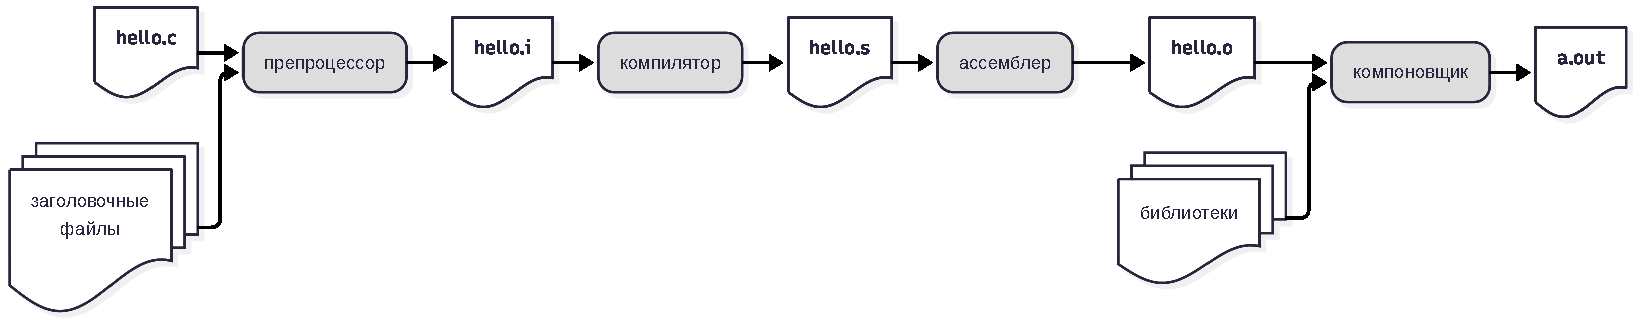
\includegraphics[width=1\linewidth]{comp_pipeline.pdf}
    \end{center}

\end{frame}

\begin{frame}[fragile]
    \frametitle{Компилятор}

    \begin{block}{hello.c}
        \inputminted{c}{workdir/hello.c}
    \end{block}

    \vspace{1em}

    \begin{minted}{console}
$ gcc -v hello.c -o hello
    \end{minted}

\end{frame}

\begin{frame}
    \frametitle{Компилятор}

    \inputminted[breaklines]{console}{gcc_-v_hello.c_trace.txt}

\end{frame}

\begin{frame}
    \frametitle{Первые выводы}

    \textbf{G}NU \textbf{C} \textbf{C}ompiler $\rightarrow$ \textbf{G}NU \textbf{C}ompiler \textbf{C}ollection

    Современный компилятор~--- набор инструментов (toolchain)

\end{frame}

\begin{frame}[fragile]
    \frametitle{Компилятор}

    \begin{minted}{console}
$ gcc -save-temps=obj hello.c -o hello
    \end{minted}

\end{frame}

\begin{frame}
    \frametitle{Формы существования кода (на Си)}

    \begin{itemize}
        \item Исходный код
        \item Ассемблер
        \item Машинный код
        \item Исполняемый код
    \end{itemize}

\end{frame}

\begin{frame}[fragile]
    \frametitle{Компилятор}

    \begin{minted}{console}
$ gcc hello.c -o hello
$ gcc -E hello.c -o hello.i
$ gcc -S hello.c -o hello.s
$ gcc -c hello.c -o hello.o
    \end{minted}

\end{frame}

\begin{frame}[fragile]
    \frametitle{Утилиты для просмотра}

    \begin{minted}{console}
$ objdump -d hello
$ hexdump -C hello
    \end{minted}

\end{frame}

\begin{frame}[fragile]
    \frametitle{Функция main}

    \begin{minted}{c}
int main() {}

int main(int argc, char *argv[]) {}
    \end{minted}

    Запускаем \texttt{./hello}

    Что будет в \texttt{argc} и \texttt{argv}?

    \vspace{1em}

    \begin{onlyenv}<2>
        \texttt{argv[0]}~--- имя программы

        \texttt{echo \$?}~--- получить последний код возврата

        Что будет, если \texttt{main} нет?
    \end{onlyenv}

\end{frame}

\begin{frame}[fragile]
    \frametitle{Линкер}

    ld~--- The GNU Linker

    \begin{itemize}
        \item Он же линковщик
        \item Он же компоновщих
        \item Он же редактор связей
    \end{itemize}

    \vspace{2em}

    Передача параметров линкеру при вызове gcc
    \begin{minted}{console}
$ gcc -Wl,-v hello.c -o hello
    \end{minted}

\end{frame}

\begin{frame}[fragile]
    \frametitle{Объявления и определения}

    Объявление (declaration)~--- указание имени функции, возвращаемого значения и принимаемых аргументов

    \vspace{1em}

    \begin{minted}{c}
int distance(int a, int b);
    \end{minted}

    \vspace{1em}

    Определение (definition)~--- выполняемая последовательность команд (тело функции)

    \vspace{1em}

    \begin{minted}{c}
int distance(int a, int b)
{
    return abs(b - a);
}
    \end{minted}

\end{frame}

\begin{frame}
    \frametitle{Домашнее задание}

    \begin{enumerate}
        \item Написать программу проверки баланса скобок в исходной строке (т.е. число открывающих скобок равно числу закрывающих и выполняется правило вложенности скобок).
              Считайте, что баланс проверяется для одного типа скобок, а строка может содержать произвольные символы
        \item Заданы две строки: S и S1.
              Найти количество вхождений S1 в S как подстроки
        \item Написать программу, считающую количество нулевых элементов в массиве
    \end{enumerate}

\end{frame}

\begin{frame}
    \frametitle{Полезные ссылки}

    \begin{itemize}
        \item Driving Compilers by Fabien Sanglard
              \begin{itemize}
                  \item \url{https://fabiensanglard.net/dc/index.php}
                  \item Серия заметок про различные части компилятора как целого
                  \item Многие слайды мотивированы именно ей
              \end{itemize}
        \item How to Compile and Run C Program in Linux Using gcc?
              \begin{itemize}
                  \item \url{https://cs-fundamentals.com/c-programming/how-to-compile-c-program-using-gcc}
              \end{itemize}
    \end{itemize}

\end{frame}

\appendix

\begin{frame}[fragile]
    \frametitle{Про домашние задания}

    \texttt{\#define <stdio.h>} и \texttt{\#define "stdio.h"} означают разные вещи

    \vspace{1em}

    \begin{minted}{console}
$ gcc -v hello.c -o hello
...
#include "..." search starts here:
#include <...> search starts here:
 /usr/lib/gcc/x86_64-pc-linux-gnu/15.2.1/include
 /usr/local/include
 /usr/lib/gcc/x86_64-pc-linux-gnu/15.2.1/include-fixed
 /usr/include
End of search list.
...
    \end{minted}
\end{frame}
\end{document}
